\PassOptionsToPackage{unicode=true}{hyperref} % options for packages loaded elsewhere
\PassOptionsToPackage{hyphens}{url}
\PassOptionsToPackage{dvipsnames,svgnames*,x11names*}{xcolor}
%
\documentclass[10pt,]{krantz}
\usepackage{lmodern}
\usepackage{amssymb,amsmath}
\usepackage{ifxetex,ifluatex}
\usepackage{fixltx2e} % provides \textsubscript
\ifnum 0\ifxetex 1\fi\ifluatex 1\fi=0 % if pdftex
  \usepackage[T1]{fontenc}
  \usepackage[utf8]{inputenc}
  \usepackage{textcomp} % provides euro and other symbols
\else % if luatex or xelatex
  \usepackage{unicode-math}
  \defaultfontfeatures{Ligatures=TeX,Scale=MatchLowercase}
    \setmonofont[Mapping=tex-ansi,Scale=0.7]{Source Code Pro}
\fi
% use upquote if available, for straight quotes in verbatim environments
\IfFileExists{upquote.sty}{\usepackage{upquote}}{}
% use microtype if available
\IfFileExists{microtype.sty}{%
\usepackage[]{microtype}
\UseMicrotypeSet[protrusion]{basicmath} % disable protrusion for tt fonts
}{}
\IfFileExists{parskip.sty}{%
\usepackage{parskip}
}{% else
\setlength{\parindent}{0pt}
\setlength{\parskip}{6pt plus 2pt minus 1pt}
}
\usepackage{xcolor}
\usepackage{hyperref}
\hypersetup{
            pdftitle={Elementos de la estadística},
            pdfauthor={Ricardo Michel MALLQUI BAÑOS},
            colorlinks=true,
            linkcolor=Maroon,
            filecolor=Maroon,
            citecolor=Blue,
            urlcolor=Blue,
            breaklinks=true}
\urlstyle{same}  % don't use monospace font for urls
\usepackage{longtable,booktabs}
% Fix footnotes in tables (requires footnote package)
\IfFileExists{footnote.sty}{\usepackage{footnote}\makesavenoteenv{longtable}}{}
\setlength{\emergencystretch}{3em}  % prevent overfull lines
\providecommand{\tightlist}{%
  \setlength{\itemsep}{0pt}\setlength{\parskip}{0pt}}
\setcounter{secnumdepth}{5}

% set default figure placement to htbp
\makeatletter
\def\fps@figure{htbp}
\makeatother

\usepackage[spanish,es-lcroman,es-tabla]{babel}
\usepackage{booktabs}
\usepackage{graphicx} 
\usepackage{amsmath}
\usepackage{makeidx}
\makeindex

\makeatletter\@addtoreset{chapter}{part}\makeatother%

\usepackage{showframe}
%\usepackage[a4paper]{geometry}
%\geometry{verbose,tmargin=3cm,bmargin=3cm,lmargin=3.5cm,rmargin=3cm}
\renewcommand{\arraystretch}{1.1}

\usepackage{times}
\renewcommand{\rmdefault}{ptm}
\usepackage[lite,subscriptcorrection,nofontinfo,zswash]{mtpro2}

\usepackage{graphicx}

% Determine if the image is too wide for the page.
\makeatletter
\def\ScaleIfNeeded{%
  \ifdim\Gin@nat@width>\linewidth
    \linewidth
  \else
    \Gin@nat@width
  \fi
}
\makeatother

% Resize figures that are too wide for the page.
\let\oldincludegraphics\includegraphics
\renewcommand\includegraphics[2][]{%
  \oldincludegraphics[scale=0.85]{#2}
}

\usepackage{amsthm}
\makeatletter
\def\thm@space@setup{%
  \thm@preskip=8pt plus 2pt minus 4pt
  \thm@postskip=\thm@preskip
}
\makeatother



\flushbottom 

\frontmatter
\usepackage[]{natbib}
\bibliographystyle{apalike}

\title{Elementos de la estadística}
\providecommand{\subtitle}[1]{}
\subtitle{estadística descriptiva y probabilidades}
\author{Ricardo Michel MALLQUI BAÑOS}
\providecommand{\institute}[1]{}
\institute{Universidad Nacional San Cristóbal De Huamanga}
\date{2020-03-30}

\usepackage{amsthm}
\newtheorem{theorem}{Teorema}[chapter]
\newtheorem{lemma}{Lema}[chapter]
\newtheorem{corollary}{Corolario}[chapter]
\newtheorem{proposition}{Proposición}[chapter]
\newtheorem{conjecture}{Conjectura}[chapter]
\theoremstyle{definition}
\newtheorem{definition}{Definición}[chapter]
\theoremstyle{definition}
\newtheorem{example}{Ejemplo}[chapter]
\theoremstyle{definition}
\newtheorem{exercise}{Ejercicio}[chapter]
\theoremstyle{remark}
\newtheorem*{remark}{Observación}
\newtheorem*{solution}{Solución}
\let\BeginKnitrBlock\begin \let\EndKnitrBlock\end
\begin{document}
\maketitle

%\cleardoublepage\newpage\thispagestyle{empty}\null
%\cleardoublepage\newpage\thispagestyle{empty}\null
%\cleardoublepage\newpage
\thispagestyle{empty}
\begin{center}
\includegraphics{U.pdf}
\end{center}

%\setlength{\abovedisplayskip}{-5pt}
%\setlength{\abovedisplayshortskip}{-5pt}

{
\hypersetup{linkcolor=}
\setcounter{tocdepth}{2}
\tableofcontents
}
\listoftables
\listoffigures
\newcommand{\N}{\mathbb{N}}
\newcommand{\R}{\mathbb{R}}
\newcommand{\CC}{\mathbb{C}}
\newcommand{\I}{\mathbb{I}}
\newcommand{\f}{\mathbb{f}}
\newcommand{\X}{\mathbb{X}}
\newcommand{\D}{\mathbb{D}}
\newcommand{\Z}{\mathbb{Z}}
\newcommand{\Q}{\mathbb{Q}}
\newcommand{\norm}[1]{\left\Vert#1\right\Vert}
\newcommand{\abs}[1]{\left\vert#1\right\vert}
\newcommand{\set}[1]{\left\{#1\right\}}
\newcommand{\seq}[1]{\left<#1\right>}
\newcommand{\co}[1]{\left[#1\right]}
\newcommand{\cc}[1]{\left(#1\right)}
\newcommand{\J}{\mathcal{J}}
\newcommand{\K}{\mathcal{K}}
\newcommand{\M}{\mathcal{M}}
\newcommand{\F}{\mathcal{F}}

\hypertarget{resumen}{%
\chapter*{Resumen}\label{resumen}}


Este libro sobre la estadistica descriptiva. cuyo objetivo es demostrar resultados basicos muy útiles en el desarrollo de investigaciones.

\[\sum_1^2\]

\hypertarget{introducciuxf3n}{%
\chapter*{Introducción}\label{introducciuxf3n}}


\[\sum_1^2\]

\[\vec{u}=(1,1)-\rho\int_2^3\]

Debido a la poca información estructurada de estadistica descriptiva se propone escribir este libro con un enfoque demostrativo.

\[x^2+y^2\]

\mainmatter

\hypertarget{part-estaduxedstica-descriptiva}{%
\part{Estadística descriptiva}\label{part-estaduxedstica-descriptiva}}

\hypertarget{prerrequisitos}{%
\chapter{Prerrequisitos}\label{prerrequisitos}}

\hypertarget{variables}{%
\chapter{Variables}\label{variables}}

Es una característica de personas cosas u objetos que sonpropensos a ser medidas
\#\# Variables cualitativas

Denotan cualidades de objetos personas o animales tales como caracteristicas inherentes que no son medibles por números, tenemos dos casos de esta variable.

\hypertarget{nominales}{%
\subsection{Nominales}\label{nominales}}

Son caracteristicas que simplemente nominan y estan propensos a ser jerarquizados u ordenados tales como: El estado civil (soltero, casado, divorciado, viudo), Religion (católic, evangelico, judio, etc).

\hypertarget{ordinales}{%
\subsection{Ordinales}\label{ordinales}}

Son caracteristicas que que si están propensos a ser jerarquizados tales como: Nivel de instrucción (primaria, secundaria, superior).

\hypertarget{variables-cuantitativas}{%
\section{Variables cuantitativas}\label{variables-cuantitativas}}

Son aqueelllas variables que están propensos a ser medidas mediante números ya sean números enteros o reales.

\hypertarget{discretas}{%
\subsection{Discretas}\label{discretas}}

Aquellas que solo son medidos mediante numeros enteros por ejemplo: Número de hijos, número de habitaciones.

\hypertarget{continuas}{%
\subsection{Continuas}\label{continuas}}

Aquellas que solo son medidos mediante numeros reales es decir este incluye a los numeros racionales e irracionales. Estatura, volumen, peso.

\hypertarget{caracteruxedstica-de-los-datos}{%
\chapter{Característica de los datos}\label{caracteruxedstica-de-los-datos}}

\hypertarget{poblaciuxf3n-muestra-y-estaduxedstica}{%
\chapter{Población, muestra y estadística}\label{poblaciuxf3n-muestra-y-estaduxedstica}}

\hypertarget{organizaciuxf3n-de-datos-en-tablas-de-frecuencias}{%
\chapter{Organización de datos en tablas de frecuencias}\label{organizaciuxf3n-de-datos-en-tablas-de-frecuencias}}

\url{https://gisanddata.maps.arcgis.com/apps/opsdashboard/index.html\#/bda7594740fd40299423467b48e9ecf6}
Sea la Tabla \ref{tab:w3} Figures and tables with captions will be placed in \texttt{figure} and \texttt{table} environments, respectively.
Figures and tables with captions will be placed in \texttt{figure} and \texttt{table} environments, respectively.
Figures and tables with captions will be placed in \texttt{figure} and \texttt{table} environments, respectively.

\begin{longtable}[t]{lrl}
\caption{\label{tab:w3}Here is a nice table!}\\
\toprule
País & z & Porcentaje\\
\midrule
Dinamarca & 8.0 & 8.00\textbackslash{}\%\\
Islandia & 7.7 & 7.70\textbackslash{}\%\\
Corea del Sur & 7.6 & 7.60\textbackslash{}\%\\
Noruega & 7.6 & 7.60\textbackslash{}\%\\
Israel & 7.4 & 7.40\textbackslash{}\%\\
Nueva Zelanda & 7.3 & 7.30\textbackslash{}\%\\
Estados Unidos & 7.3 & 7.30\textbackslash{}\%\\
Bélgica & 6.6 & 6.60\textbackslash{}\%\\
Canada & 6.6 & 6.60\textbackslash{}\%\\
Finlandia & 6.5 & 6.50\textbackslash{}\%\\
Suecia & 6.5 & 6.50\textbackslash{}\%\\
Reino Unido & 6.5 & 6.50\textbackslash{}\%\\
Chile & 6.4 & 6.40\textbackslash{}\%\\
Irlanda & 6.4 & 6.40\textbackslash{}\%\\
Francia & 6.3 & 6.30\textbackslash{}\%\\
Holanda & 6.3 & 6.30\textbackslash{}\%\\
Mexico & 6.2 & 6.20\textbackslash{}\%\\
Australia & 6.1 & 6.10\textbackslash{}\%\\
Estonia & 6.0 & 6.00\textbackslash{}\%\\
Eslovenia & 5.9 & 5.90\textbackslash{}\%\\
Austria & 5.8 & 5.80\textbackslash{}\%\\
Polonia & 5.8 & 5.80\textbackslash{}\%\\
Portugal & 5.8 & 5.80\textbackslash{}\%\\
España & 5.6 & 5.60\textbackslash{}\%\\
Suiza & 5.6 & 5.60\textbackslash{}\%\\
Japón & 5.1 & 5.10\textbackslash{}\%\\
Alemania & 5.0 & 5.00\textbackslash{}\%\\
República Checa & 4.7 & 4.70\textbackslash{}\%\\
Italia & 4.7 & 4.70\textbackslash{}\%\\
Hungria & 4.6 & 4.60\textbackslash{}\%\\
Eslovaquia & 4.6 & 4.60\textbackslash{}\%\\
Grecia & 4.3 & 4.30\textbackslash{}\%\\
\bottomrule
\end{longtable}

\begin{longtable}[t]{lccrrlc}
\caption{\label{tab:ww3}Here!}\\
\toprule
ID & Motivador & X3 & $\overline{x}$ & Formativa & X6 & X7\\
\midrule
 & IT1 & IT2 & O1 & IT3 & IT4 & IT5\\
1 & 2 & 2 & 2 & 2 & 1 & 1\\
2 & 3 & 2 & 3 & 3 & 3 & 3\\
3 & 3 & 3 & 3 & 3 & 2 & 2\\
4 & 3 & 3 & 3 & 2 & 2 & 2\\
5 & 3 & 2 & 3 & 3 & 3 & 3\\
6 & 1 & 1 & 1 & 1 & 2 & 2\\
7 & 2 & 3 & 3 & 3 & 3 & 2\\
8 & 2 & 2 & 2 & 1 & 1 & 1\\
9 & 1 & 2 & 2 & 1 & 1 & 1\\
10 & 1 & 2 & 2 & 2 & 1 & 1\\
11 & 2 & 2 & 2 & 2 & 2 & 2\\
12 & 2 & 3 & 3 & 3 & 2 & 2\\
13 & 3 & 2 & 3 & 3 & 2 & 2\\
14 & 2 & 3 & 3 & 2 & 2 & 3\\
15 & 2 & 2 & 2 & 2 & 2 & 1\\
16 & 2 & 2 & 2 & 3 & 2 & 3\\
17 & 2 & 2 & 2 & 2 & 2 & 2\\
18 & 1 & 2 & 2 & 1 & 1 & 2\\
19 & 3 & 2 & 3 & 3 & 3 & 3\\
20 & 3 & 3 & 3 & 3 & 2 & 2\\
21 & 1 & 1 & 1 & 1 & 2 & 2\\
22 & 3 & 3 & 3 & 3 & 3 & 2\\
23 & 3 & 2 & 3 & 3 & 3 & 3\\
24 & 3 & 2 & 3 & 3 & 3 & 3\\
25 & 2 & 3 & 3 & 3 & 3 & 2\\
26 & 2 & 2 & 2 & 1 & 1 & 1\\
27 & 1 & 2 & 2 & 1 & 2 & 2\\
28 & 3 & 2 & 3 & 3 & 2 & 2\\
29 & 3 & 2 & 3 & 3 & 3 & 3\\
30 & 1 & 2 & 2 & 2 & 1 & 1\\
31 & 3 & 3 & 3 & 3 & 3 & 2\\
32 & 3 & 3 & 3 & 2 & 3 & 3\\
33 & 1 & 1 & 1 & 1 & 1 & 1\\
34 & 1 & 1 & 1 & 1 & 1 & 1\\
35 & 3 & 2 & 3 & 2 & 2 & 2\\
 & $\sum_{i=1}^nx_i$ &  &  &  &  & \\
\bottomrule
\end{longtable}

\begin{longtable}[t]{llllllll}
\caption{\label{tab:unnamed-chunk-1}Figures and tables with captions will be placed in `figure`}\\
\toprule
  & X1 & $\alpha$ & $\sum^{n}_{i=1}{x_i}$ & X4 & X5 & X6 & X7\\
\midrule
1 & ID & Motivador &  & $\overline{x}$ & Formativa &  & \\
2 &  & IT1 & IT2 & O1 & IT3 & IT4 & IT5\\
3 & 1 & 2 & 2 & 2 & 2 & 1 & 1\\
4 & 2 & 3 & 2 & 3 & 3 & 3 & 3\\
5 & 3 & 3 & 3 & 3 & 3 & 2 & 2\\
6 & 4 & 3 & 3 & 3 & 2 & 2 & 2\\
$\beta_0$ & 5 & 3 & 2 & 3 & 3 & 3 & 3\\
$\beta_1$ & 6 & 1 & 1 & 1 & 1 & 2 & 2\\
$\beta_3$ & 7 & 2 & 3 & 3 & 3 & 3 & 2\\
10 & 8 & 2 & 2 & 2 & 1 & 1 & 1\\
11 & 9 & 1 & 2 & 2 & 1 & 1 & 1\\
12 & 10 & 1 & 2 & 2 & 2 & 1 & 1\\
13 & 11 & 2 & 2 & 2 & 2 & 2 & 2\\
14 & 12 & 2 & 3 & 3 & 3 & 2 & 2\\
15 & 13 & 3 & 2 & 3 & 3 & 2 & 2\\
16 & 14 & 2 & 3 & 3 & 2 & 2 & 3\\
17 & 15 & 2 & 2 & 2 & 2 & 2 & 1\\
18 & 16 & 2 & 2 & 2 & 3 & 2 & 3\\
19 & 17 & 2 & 2 & 2 & 2 & 2 & 2\\
20 & 18 & 1 & 2 & 2 & 1 & 1 & 2\\
21 & 19 & 3 & 2 & 3 & 3 & 3 & 3\\
22 & 20 & 3 & 3 & 3 & 3 & 2 & 2\\
23 & 21 & 1 & 1 & 1 & 1 & 2 & 2\\
24 & 22 & 3 & 3 & 3 & 3 & 3 & 2\\
25 & 23 & 3 & 2 & 3 & 3 & 3 & 3\\
26 & 24 & 3 & 2 & 3 & 3 & 3 & 3\\
27 & 25 & 2 & 3 & 3 & 3 & 3 & 2\\
28 & 26 & 2 & 2 & 2 & 1 & 1 & 1\\
29 & 27 & 1 & 2 & 2 & 1 & 2 & 2\\
30 & 28 & 3 & 2 & 3 & 3 & 2 & 2\\
31 & 29 & 3 & 2 & 3 & 3 & 3 & 3\\
32 & 30 & 1 & 2 & 2 & 2 & 1 & 1\\
33 & 31 & 3 & 3 & 3 & 3 & 3 & 2\\
34 & 32 & 3 & 3 & 3 & 2 & 3 & 3\\
$\sum^{n}_{i=1}{x_i}$ & 33 & 1 & 1 & 1 & 1 & 1 & 1\\
36 & 34 & 1 & 1 & 1 & 1 & 1 & 1\\
37 & 35 & 3 & 2 & 3 & 2 & 2 & 2\\
38 &  & $\sum_{i=1}^nx_i$ &  &  &  &  & \\
\bottomrule
\end{longtable}

Figures and tables with captions will be placed in \texttt{figure} and \texttt{table} environments, respectively Figura \ref{fig:www}

\begin{figure}

{\centering 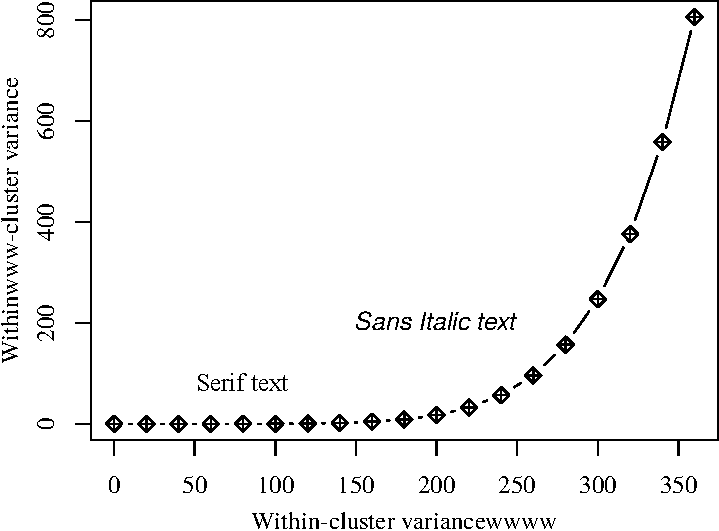
\includegraphics{E_1_files/figure-latex/www-1} 

}

\caption{Here is a nice figure 100!}\label{fig:www}
\end{figure}

\begin{figure}

{\centering 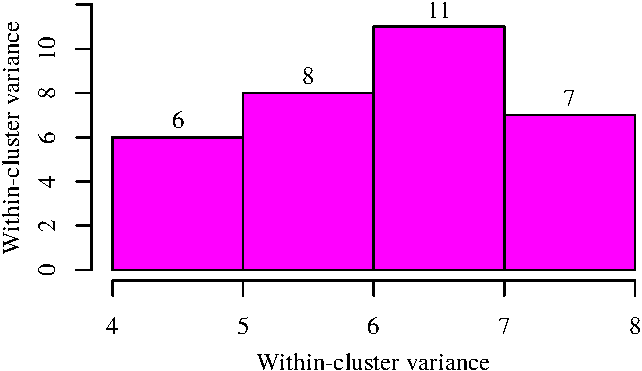
\includegraphics{E_1_files/figure-latex/wwwww-1} 

}

\caption{Here is a nice figure 100!}\label{fig:wwwww}
\end{figure}

Centering

\hypertarget{matriz-y-rango}{%
\chapter{Matriz y rango}\label{matriz-y-rango}}

\hypertarget{distribuciuxf3-n-de-frecuencias}{%
\chapter{Distribució n de frecuencias}\label{distribuciuxf3-n-de-frecuencias}}

La tabulación es un proceso en el cual los datos son ordenados en grupos llamados \emph{clases} para un análisis más eficaz de estos, los datos podrían estar clasificados mediante una variable cualitativa o cuantitativa en el caso de las variables cualitativas \(Y_i\), se considera la siguiente Tabla \ref{tab:ww}

\begin{longtable}[]{@{}cccccccccc@{}}
\caption{\label{tab:ww} Caption}\tabularnewline
\toprule
\(Y_i\) & \(f_i\) & \(F_i\) & \(F_i^*\) & \(h_i\) & \(H_i\) & \(H_i^*\) & \(h_i\%\) & \(H_i\%\) & \(H_i^*\%\)\tabularnewline
\midrule
\endfirsthead
\toprule
\(Y_i\) & \(f_i\) & \(F_i\) & \(F_i^*\) & \(h_i\) & \(H_i\) & \(H_i^*\) & \(h_i\%\) & \(H_i\%\) & \(H_i^*\%\)\tabularnewline
\midrule
\endhead
\(Y_1\) & \(f_1\) & \(F_1\) & \(F_1^*\) & \(\frac{f_1}{n}\) & \(\frac{F_1}{n}\) & \(\frac{F_1^*}{n}\) & \(h_1\) & \(H_1\) & \(H_1^*\)\tabularnewline
\(Y_2\) & \(f_2\) & \(F_2\) & \(F_2^*\) & \(\frac{f_2}{n}\) & \(\frac{F_2}{n}\) & \(\frac{F_2^*}{n}\) & \(h_2\) & \(H_2\) & \(H_1^*\)\tabularnewline
\(Y_3\) & \(f_3\) & \(F_3\) & \(F_3^*\) & \(\frac{f_3}{n}\) & \(\frac{F_3}{n}\) & \(\frac{F_3^*}{n}\) & \(h_3\) & \(H_3\) & \(H_1^*\)\tabularnewline
\(\vdots\) & \(\vdots\) & \(\vdots\) & \(\vdots\) & \(\vdots\) & \(\vdots\) & \(\vdots\) & \(\vdots\) & \(\vdots\) & \(\vdots\)\tabularnewline
\(Y_r\) & \(f_r\) & \(F_r\) & \(F_r^*\) & \(\frac{f_r}{n}\) & \(\frac{F_r}{n}\) & \(\frac{F_r^*}{n}\) & \(h_r\) & \(H_r\) & \(H_1^*\)\tabularnewline
\bottomrule
\end{longtable}

En el caso de variables cuantitativas ademas si los datos son muy variados, que para se clasificados adecuadamente, necesitan generarse particiones de longitudes semejantes entonces se utiliza el siguiente proceso; el \textbf{número de las particiones} \(r\) se consideran de acuerdo a \textbf{tres criterios}

\begin{itemize}
\item
  Criterio del investigador \(r\) no puede ser más de 20 ni menos de 5
\item
  \(r=\sqrt{n}\) donde \(n\) es el número de datos
\item
  La regla de Starges que consiste en considerar la fórmula \(r=3.322\cdot\log_{10} n\)
  Una vez establecido el número de particiones se procede a generar los límites laterales de cada una de las particiones, sea \(L\) la longitud de todo el conjunto es decir \(L=x_{\text{max}}-x_{\text{min}}\) entonces la longitud de las particiones o amplitud interválica se obtiene con \(l=\frac{L}{r}\)
\end{itemize}

\begin{longtable}[]{@{}ccccccccc@{}}
\toprule
Clase & Clase & \(f_i\) & \(F_i\) & \(F_i^*\) & \(h_i\) & \(H_i\) & \(H_i^*\) & \(\ldots\)\tabularnewline
\midrule
\endhead
\([y_1-y_2>\) & \(y_1\) & \(f_1\) & \(F_1\) & \(F_1^*\) & \(\frac{f_1}{n}\) & \(\frac{F_1}{n}\) & \(\frac{F_1^*}{n}\) & \(\ldots\)\tabularnewline
\(<y_1-y_2>\) & \(y_2\) & \(f_2\) & \(F_2\) & \(F_2^*\) & \(\frac{f_2}{n}\) & \(\frac{F_2}{n}\) & \(\frac{F_2^*}{n}\) & \(\ldots\)\tabularnewline
\(<y_{r}-y_r>\) & \(y_3\) & \(f_3\) & \(F_3\) & \(F_3^*\) & \(\frac{f_3}{n}\) & \(\frac{F_3}{n}\) & \(\frac{F_3^*}{n}\) & \(\ldots\)\tabularnewline
\(\vdots\) & \(\vdots\) & \(\vdots\) & \(\vdots\) & \(\vdots\) & \(\vdots\) & \(\vdots\) & \(\vdots\) & \(\vdots\)\tabularnewline
\(<y_{r-1}-y_r]\) & \(y_r\) & \(f_r\) & \(F_r\) & \(F_r^*\) & \(\frac{f_r}{n}\) & \(\frac{F_r}{n}\) & \(\frac{F_r^*}{n}\) & \(...\)\tabularnewline
\bottomrule
\end{longtable}

Tenga en cuenta que \(n\) es el número de datos, es decir \(n=f_1+f_2+\ldots+f_r=\sum_{i=1}^r\) donde \(f_i\) es número de datos en la partición \(X_i\), una de las \(r\) particiones del conjunto total de datos.

\begin{itemize}
\item
  Las \textbf{frecuencias absolutas}\index{frecuencias absolutas} \(f_i\) indican el número de datos con la característica \(X_i\).
\item
  Las \textbf{frecuencias absolutas acumuladas menor que}\index{frecuencias absolutas acumuladas menor que} \(F_i\) obedecen a la fórmula
  \[F_m=f_1+f_2+\ldots+f_m=\sum_{i=1}^mf_i\]
\item
  Las \textbf{frecuencias absolutas acumuladas mayor que} \(F_i^*\) obedecen a la fórmula
  \[F_m^*=f_m+f_{m+1}+\ldots+f_r=\sum_{i=m}^rf_i=n-\sum_{i=1}^{m-1}f_i=n-\left(f_1+f_{2}+\ldots+f_{m-1}\right)\]
\item
  Las \textbf{frecuencias absolutas relativas}\index{frecuencias absolutas relativas} obedecen a la fórmula
  \[h_m=\frac{f_m}{n}\]
\item
  Las \textbf{frecuencias absolutas relativas menor que}\index{frecuencias absolutas relativas  menor que} obedecen a la fórmula
  \[H_m=\frac{f_m}{n}\]
\item
  Las \textbf{frecuencias absolutas relativas mayor que} obedecen a la fórmula
  \[H_m^*=\frac{F_m}{n}\]
\item
  Las \textbf{frecuencias absolutas relativas porcentuales} obedecen a la fórmula
  \(h_i\%=100\cdot h_i\)
\item
  Las \textbf{frecuencias absolutas relativas menor que porcentuales} obedecen a la fórmula
  \(H_i\%=100\cdot H_i\)
\item
  Las \textbf{frecuencias absolutas relativas mayor que porcentuales} obedecen a la fórmula
  \(H_i^*\%=100\cdot H_i^*\)
\end{itemize}

\BeginKnitrBlock{exercise}
\protect\hypertarget{exr:unnamed-chunk-2}{}{\label{exr:unnamed-chunk-2} }Sean los datos
\EndKnitrBlock{exercise}

\BeginKnitrBlock{solution}
\iffalse{} {Solución. } \fi{}Entonces
\EndKnitrBlock{solution}

\hypertarget{gruxe1ficos-estaduxedsticos}{%
\chapter{Gráficos estadísticos}\label{gruxe1ficos-estaduxedsticos}}

\hypertarget{medidas-de-tendencia-central}{%
\chapter{Medidas de tendencia central}\label{medidas-de-tendencia-central}}

Son aquellas medidas que buscan un dato representtivo central de un conjunto de datos tales como la media, la moda y la mediana.

\hypertarget{la-media-overlinex}{%
\section{\texorpdfstring{La media (\(\overline{x}\))}{La media (\textbackslash{}overline\{x\})}}\label{la-media-overlinex}}

A veces llamada \emph{promedio aritmético}, es la medida de tendencia central que pondera los datos.

\hypertarget{media-de-datos-no-agrupados}{%
\subsection{Media de datos no agrupados}\label{media-de-datos-no-agrupados}}

Los datos no están agrupados cuando no están ordenados sobre una tabla de distribución de frecuencias. Sean los \(n\) datos \(x_1, x_2,\ldots, x_n\) entonces la media o promedio aritmético se define como
\begin{equation}
\overline{x}=\frac{x_1+x_2+\cdots+x_n}{n}=\frac{1}{n}\sum_{i=1}^nx_i
\label{eq:w1}
\end{equation}
\begin{equation}
\frac{d\left[P;F_1\right]}{d\left[P;\mathcal{L}_1\right]}=e=\frac{d\left[P;F_2\right]}{d\left[P;\mathcal{L}_2\right]}
\label{eq:ww}
\end{equation}

\begin{enumerate}
\def\labelenumi{\arabic{enumi}.}
\tightlist
\item
  \(\overline{x}=\frac{x_1+x_2+\cdots+x_n}{n}=\frac{1}{n}\sum_{i=1}^nx_i\)
\item
  \(\overline{x}=\frac{x_1+x_2+\cdots+x_n}{n}=\frac{1}{n}\sum_{i=1}^nx_i\)
\end{enumerate}

\hypertarget{media-de-datos-agrupados}{%
\subsection{Media de datos agrupados}\label{media-de-datos-agrupados}}

Considérese la siguiente tabla de distribucion de frecuencias entonces el promedio es \[\overline{x}=\frac{y_1f_1+y_2f_2+\cdots+y_nf_n}{n}=\frac{1}{n}\sum_{i=1}^ny_if_i\]

\begin{longtable}[]{@{}ccccccccc@{}}
\toprule
Clase & Clase & \(f_i\) & \(F_i\) & \(F_i^*\) & \(h_i\) & \(H_i\) & \(H_i^*\) & \(\ldots\)\tabularnewline
\midrule
\endhead
\(<y_1-y_2>\) & \(y_1\) & \(f_1\) & \(F_1\) & \(F_1^*\) & \(\frac{f_1}{n}\) & \(\frac{F_1}{n}\) & \(\frac{F_1^*}{n}\) & \(\ldots\)\tabularnewline
\(<y_2-y_3>\) & \(y_2\) & \(f_2\) & \(F_2\) & \(F_2^*\) & \(\frac{f_2}{n}\) & \(\frac{F_2}{n}\) & \(\frac{F_2^*}{n}\) & \(\ldots\)\tabularnewline
\(<y_3-y_4>\) & \(y_3\) & \(f_3\) & \(F_3\) & \(F_3^*\) & \(\frac{f_3}{n}\) & \(\frac{F_3}{n}\) & \(\frac{F_3^*}{n}\) & \(\ldots\)\tabularnewline
\(\vdots\) & \(\vdots\) & \(\vdots\) & \(\vdots\) & \(\vdots\) & \(\vdots\) & \(\vdots\) & \(\vdots\) & \(\vdots\)\tabularnewline
\(<y_{r-1}-y_r]\) & \(y_r\) & \(f_r\) & \(F_r\) & \(F_r^*\) & \(\frac{f_r}{n}\) & \(\frac{F_r}{n}\) & \(\frac{F_r^*}{n}\) & \(...\)\tabularnewline
\bottomrule
\end{longtable}

\BeginKnitrBlock{exercise}
\protect\hypertarget{exr:unnamed-chunk-4}{}{\label{exr:unnamed-chunk-4} }Si el promedio de \(n\) datos es \(\overline{x}\) entonces el promedio del conjunto inicial más un dato adicional \(x_{n+1}\) es \[\overline{x}'=\frac{n\overline{x}+x_{n+1}}{n+1}\] en general si se adicionan \(r\) datos \(y_1, y_2, \ldots y_r\) entonces el nuevo promedio será \[\overline{x}'=\frac{n\overline{x}+y_{1}+y_2+\ldots+y_r}{n+r}\]
\EndKnitrBlock{exercise}

\BeginKnitrBlock{solution}
\iffalse{} {Solución. } \fi{}En efecto sea el promedio
\begin{align*}
\overline{x}'&=\frac{x_1+x_2+\cdots+x_{n+1}}{n+1}\\
&=\frac{n\frac{x_1+x_2+\cdots x_n}{n}+x_{n+1}}{n+1}\\
&=\frac{n\overline{x}+x_{n+1}}{n+1}
\end{align*}
\EndKnitrBlock{solution}

\hypertarget{la-moda-mo}{%
\section{La moda (Mo)}\label{la-moda-mo}}

\hypertarget{moda-de-datos-no-tabulados}{%
\subsection{Moda de datos no tabulados}\label{moda-de-datos-no-tabulados}}

En este caso es dato que más repite en un conjunto de datos dados.

La moda es el dato que más se repite por ejemplo sea el conjunto de datos \(x_1,\) \(x_2,\) \(x_2,\) \(x_2,\) \(x_3\) entonces la moda \(\text{Mo}=x_2\)

\hypertarget{moda-de-datos-tabulados}{%
\subsection{Moda de datos tabulados}\label{moda-de-datos-tabulados}}

La moda es el dato que más se repite por ejemplo sea el conjunto de datos \(x_1,\) \(x_2,\) \(x_2,\) \(x_2,\) \(x_3\) entonces la moda \(\text{Mo}=Li+\frac{Li-Ls}{Li+Ls}r\)

\begin{longtable}[]{@{}ccccccccc@{}}
\toprule
Clase & Clase & \(f_i\) & \(F_i\) & \(F_i^*\) & \(h_i\) & \(H_i\) & \(H_i^*\) & \(\ldots\)\tabularnewline
\midrule
\endhead
\([y_1-y_2>\) & \(y_1\) & \(f_1\) & \(F_1\) & \(F_1^*\) & \(\frac{f_1}{n}\) & \(\frac{F_1}{n}\) & \(\frac{F_1^*}{n}\) & \(\ldots\)\tabularnewline
\(<y_1-y_2>\) & \(y_2\) & \(f_2\) & \(F_2\) & \(F_2^*\) & \(\frac{f_2}{n}\) & \(\frac{F_2}{n}\) & \(\frac{F_2^*}{n}\) & \(\ldots\)\tabularnewline
\(<y_{r}-y_r>\) & \(y_3\) & \(f_3\) & \(F_3\) & \(F_3^*\) & \(\frac{f_3}{n}\) & \(\frac{F_3}{n}\) & \(\frac{F_3^*}{n}\) & \(\ldots\)\tabularnewline
\(\vdots\) & \(\vdots\) & \(\vdots\) & \(\vdots\) & \(\vdots\) & \(\vdots\) & \(\vdots\) & \(\vdots\) & \(\vdots\)\tabularnewline
\(<y_{r-1}-y_r]\) & \(y_r\) & \(f_r\) & \(F_r\) & \(F_r^*\) & \(\frac{f_r}{n}\) & \(\frac{F_r}{n}\) & \(\frac{F_r^*}{n}\) & \(...\)\tabularnewline
\bottomrule
\end{longtable}

\hypertarget{la-mediana-me}{%
\section{la mediana (Me)}\label{la-mediana-me}}

\hypertarget{mediana-de-datos-no-tabulados}{%
\subsection{Mediana de datos no tabulados}\label{mediana-de-datos-no-tabulados}}

Obtener la mediana consiste en ordenar los datos de menor a mayor y considerar dos casos: El prmero si el numero de datos s impar entonces el dato \(x_{\frac{n+1}{2}}\) del conjunto ordenado será la mediana es decir \(\text{Me}=x_{\frac{n+1}{2}}\) de otro lado si el número de datos es par entonces la mediana es la semisuma de los dos datos intermedios es decir \(\text{Me}=\frac{x_{\frac{n}{2}}+x_{\frac{n}{2}+1}}{2}\)

\BeginKnitrBlock{exercise}
\protect\hypertarget{exr:unnamed-chunk-6}{}{\label{exr:unnamed-chunk-6} }Sean los conjuntos de datos 5, 6, 8, 2, 1, 5, 6, 7, 10, 0, 14 y 20, 25, 6, 5, 19, 5 obtener la mediana de estos conjuntos de datos.
\EndKnitrBlock{exercise}

\BeginKnitrBlock{solution}
\iffalse{} {Solución. } \fi{}Al ordenarlos se obtiene el siguiente arreglo 0, 1, 2, 5, 5, 6, 6, 7, 8, 10, 14 y considerando que \(x_1=0\), \(x_2=1\), \(\ldots\), \(x_{11}=14\) en este caso el número de datos es impar entonces el dato \(x_{\frac{11+1}{2}}=x_{6}=6\) el la mediana. De otro lado el segundo conjunto de datos al ser ordenados 5, 5, 6, 19, 20, 25 ademas considerando que \(x_1=5\), \(x_2=5\), \(\ldots\), \(x_6=25\) conducen a obtener la mediana \(\text{Me}=\frac{x_{\frac{6}{2}}+x_{\frac{6}{2}+1}}{2}=\frac{6+19}{2}=12.5\).
\EndKnitrBlock{solution}

\hypertarget{mediana-de-datos-tabulados}{%
\subsection{Mediana de datos tabulados}\label{mediana-de-datos-tabulados}}

\begin{longtable}[]{@{}ccccccccc@{}}
\toprule
Clase & Clase & \(f_i\) & \(F_i\) & \(F_i^*\) & \(h_i\) & \(H_i\) & \(H_i^*\) & \(\ldots\)\tabularnewline
\midrule
\endhead
\([y_1-y_2>\) & \(y_1\) & \(f_1\) & \(F_1\) & \(F_1^*\) & \(\frac{f_1}{n}\) & \(\frac{F_1}{n}\) & \(\frac{F_1^*}{n}\) & \(\ldots\)\tabularnewline
\(<y_1-y_2>\) & \(y_2\) & \(f_2\) & \(F_2\) & \(F_2^*\) & \(\frac{f_2}{n}\) & \(\frac{F_2}{n}\) & \(\frac{F_2^*}{n}\) & \(\ldots\)\tabularnewline
\(<y_{r}-y_r>\) & \(y_3\) & \(f_3\) & \(F_3\) & \(F_3^*\) & \(\frac{f_3}{n}\) & \(\frac{F_3}{n}\) & \(\frac{F_3^*}{n}\) & \(\ldots\)\tabularnewline
\(\vdots\) & \(\vdots\) & \(\vdots\) & \(\vdots\) & \(\vdots\) & \(\vdots\) & \(\vdots\) & \(\vdots\) & \(\vdots\)\tabularnewline
\(<y_{r-1}-y_r]\) & \(y_r\) & \(f_r\) & \(F_r\) & \(F_r^*\) & \(\frac{f_r}{n}\) & \(\frac{F_r}{n}\) & \(\frac{F_r^*}{n}\) & \(...\)\tabularnewline
\bottomrule
\end{longtable}

Los pasos son:

\begin{itemize}
\tightlist
\item
  Se halla \(\frac{n}{2}\) luego
\item
  \(x_n\)
\item
  \[ \begin{pmatrix}
  1&1&1&1\\
  1&1&1&1\\
  1&1&1&1
  \end{pmatrix}\]
  can be found on the Pandoc website \url{http://pandoc.org}.
  \[\sum\]
  \textgreater{} I thoroughly disapprove of duels. If a man should challenge me,
  I would take him kindly and forgivingly by the hand and lead him
  to a quiet place and kill him.
\end{itemize}

In this section, we give a very brief introduction to Pandoc's Markdown. Readers who are familiar with Markdown can skip this section. The comprehensive syntax of Pandoc's Markdown can be found on the Pandoc website \url{http://pandoc.org}. \(\sum_1^2\)

\begin{quote}
I thoroughly disapprove of duels. If a man should challenge me,
I would take him kindly and forgivingly by the hand and lead him
to a quiet place and kill him.

-- Mark Twain
\end{quote}

\[\begin{pmatrix}\alpha & \beta\\
\gamma & \delta
\end{pmatrix}-\frac{2}{3} \begin{pmatrix}\alpha_1 & \beta_2\\
\gamma & \delta
\end{pmatrix}\]
* La suma de dos matrices \(A_{n\times m}\) y \(B_{r\times s}\) \[A_{n\times m}\pm B_{n\times m}=[a_{ij}+b_{ij}]\]
* El producto de dos matrices \(A_{n\times m}\) y \(B_{r\times s}\) \[A_{n\times m}\cdot B_{n\times m}=[a_{ij}+b_{ij}]\]
\[X = \begin{bmatrix}1 & x_{1}\\
1 & x_{2}\\
1 & x_{3}
\end{bmatrix}\]

\[\begin{vmatrix}a & b\\
c & d
\end{vmatrix}=ad-bc\]

\[\begin{array}{ccc}
x_{11} & x_{12} & x_{13}\\
x_{21} & x_{22} & x_{23}
\end{array}\]

\hypertarget{medidas-de-dispersiuxf3n}{%
\chapter{Medidas de dispersión}\label{medidas-de-dispersiuxf3n}}

\hypertarget{medidas-de-asimetruxeda}{%
\chapter{Medidas de asimetría}\label{medidas-de-asimetruxeda}}

\hypertarget{part-probabilidades}{%
\part{Probabilidades}\label{part-probabilidades}}

\hypertarget{frecuencia-relativa-cluxe1sica}{%
\chapter{Frecuencia relativa clásica}\label{frecuencia-relativa-cluxe1sica}}

\hypertarget{calculando}{%
\chapter{Calculando}\label{calculando}}

\hypertarget{variable-aleatoria}{%
\chapter{Variable aleatoria}\label{variable-aleatoria}}

\hypertarget{variable-acumulativa}{%
\chapter{Variable acumulativa}\label{variable-acumulativa}}

\hypertarget{ww}{%
\chapter{ww}\label{ww}}

\hypertarget{appendix-apendice}{%
\appendix \addcontentsline{toc}{chapter}{\appendixname}}


\hypertarget{sumatorias}{%
\chapter{Sumatorias}\label{sumatorias}}

Una suma de números representados por \(x_1, x_2, \ldots, x_n\) se simboliza en forma compacta mediante el simbolo \(\sum\) (sigma) es decir la suma de los números anteriores se puede escribir del siguiente modo \[x_1+x_2+\dots+x_n=\sum_{i=1}^nx_i.\]
Algunas propiedades son

\begin{enumerate}
\def\labelenumi{\arabic{enumi}.}
\tightlist
\item
  \(k\sum_{i=1}^nx_i=\sum_{i=1}^nkx_i\)
\item
  \(\sum_{i=1}^n\left(x_i+y_i\right)=\sum_{i=1}^nx_i+\sum_{i=1}^ny_i\)
\item
  \(\sum_{i=1}^nx_i\)
  \[\int_1^3=\lim_{n\to \infty}\sum_{i=0}^{n}f^i(x)\]
  citado por \citep{xie2015}
\end{enumerate}

\hypertarget{ee}{%
\section{ee}\label{ee}}

\hypertarget{eeeee}{%
\section{eeeee}\label{eeeee}}

\hypertarget{matrices}{%
\chapter{Matrices}\label{matrices}}

Una matriz es un arreglo de números distribuidos en filas y columnas por ejemplo la siguiente matriz
\[A=\begin{pmatrix}
a_{11}&a_{12}&\ldots&a_{1n}\\
a_{21}&a_{22}&\ldots&a_{2n}\\
\vdots & \vdots & \ddots &\vdots \\
a_{11}&a_{11}&\ldots&a_{nm}
\end{pmatrix}_{n\times n}\]
de \textbf{orden} \(n\times m\) tiene \textbf{entradas} \(a_{ij}\) donde el primer subindice indica la fila y el segundo la columna; es usual representar por simplicidad una matriz por \(A=[a_{ij}]_{n\times m}\). Si en el orden \(n=m\) entonces la matriz recibe el nombre de \textbf{matriz cuadrada} la suma de los elementos de la diagonal de una matriz cuadrada \(\sum_{i=1}^na_{ii}\) se llama \textbf{traza}\index{traza}. Si todas las \(a_{ij}\) son cero entonces la matriz \(A=0\) recibe el nombre matriz \textbf{nula}.

Dos matrices son iguales si tienen el \textbf{mismo orden} y cada una de las entradas respectivas son iguales es decir \(A=[a_{ij}]_{n\times m}\) y \(B=[b_{ij}]_{n\times m}\) son iguales si \(a_{ij}=b_{ij}\), \(i=1,2,\ldots n\) y \(j=1,2,\ldots m\)

\hypertarget{algebra-de-matrices}{%
\section{Algebra de matrices}\label{algebra-de-matrices}}

Sean las matrices \(A=[a_{ij}]_{n\times m}\) y \(B=[b_{ij}]_{p\times q}\) entonces la suma y producto de matrices se definen

\begin{enumerate}
\def\labelenumi{\arabic{enumi}.}
\item
  Sea \(k\) un escalar entonces se verifica que \(kA=[ka_{ij}]\), \(i=1,2,\ldots n\) y \(j=1,2,\ldots m\) es decir el escalar \(k\) multiplica a cada una de las entradas de la matriz.
\item
  La suma o diferencia es posible si \(n=p\) y \(m=q\) es decir los ordenes de \(A\) y \(B\) son iguales, entonces la suma o diferencia resulta \(A\pm B=[a_{ij}+b_{ij}]_{n\times m}\), \(i=1,2,\ldots n\) y \(j=1,2,\ldots m\)
\item
  El producto es posible si \(m=p\) es decir el número columnas de la primera matriz es igual al número de filas de la segunda matriz, el orden de la matriz resultante es \(n\times q\) además
  \begin{align*}
  A\cdot B&=\left[\sum_{k=1}^pa_{ik}b_{kj}\right]_{n\times q}\\
  &=\begin{pmatrix}
  \sum_{k=1}^ma_{1k}b_{k1}&\sum_{k=1}^ma_{1k}b_{k2}&\ldots&\sum_{k=1}^ma_{1k}b_{kq}\\
  \sum_{k=1}^ma_{2k}b_{k1}&\sum_{k=1}^ma_{2k}b_{k2}&\ldots&\sum_{k=1}^ma_{2k}b_{kq}\\
  \vdots & \vdots & \ddots &\vdots \\
  \sum_{k=1}^ma_{nk}b_{k1}&\sum_{k=1}^ma_{nk}b_{k2}&\ldots&\sum_{k=1}^ma_{nk}b_{kq}\\
  \end{pmatrix}_{n\times q}
  \end{align*}
\end{enumerate}

donde \(i=1,2,\ldots n\) y \(j=1,2,\ldots m\)

\BeginKnitrBlock{example}
\protect\hypertarget{exm:unnamed-chunk-8}{}{\label{exm:unnamed-chunk-8} }Sean \(\begin{pmatrix} 3&-1&2\\ 2&-1&2\\ 1&-1&0\\ 5&0&0\\ \end{pmatrix}_{4\times 3}\) y \(\begin{pmatrix} 0&-1&2&2&0\\ 1&-1&-2&1&1\\ 3&-1&-3&5&2\\ \end{pmatrix}_{3\times 5}\) entonces \(A\cdot B=\begin{pmatrix} 5&-4&2&15&3\\ 5&-3&0&13&3\\ -1&0&4&1&-1\\ 0&-5&10&10&0\\ \end{pmatrix}_{4\times 5}\)
\EndKnitrBlock{example}

En caso de ser posible la multiplicación entre \(A\), \(B\) y \(C\) entonces se verfican las siguientes propiedades

\begin{itemize}
\tightlist
\item
  \(A(B+C)=AB+AC\)
\item
  \((A+B)C\)
\item
  \(A(BC)=(AB)C\)
\end{itemize}

\bibliography{book.bib,packages.bib}

\printindex

\end{document}
